% \documentclass[bwprint]{cumcmthesis} %去掉封面与编号页
\documentclass[withoutpreface,bwprint]{cumcmthesis} %去掉封面与编号页
\newcommand{\diff}{\mathop{}\!\mathrm{d}} % 正体微分符号

\usepackage{graphicx}       % 用于插入图片
\usepackage{subcaption} 
\usepackage{algorithm}
\usepackage{algorithmic} % 导言区需添加这两个宏包
\usepackage{comment}  

\usepackage{booktabs}
\usepackage{tabularx}
\usepackage{float}
\usepackage[numbers]{natbib}

\title{基于统计学习方法的NIPT时点选择与胎儿的异常判定决策模型}
\tihao{C}
\baominghao{1234}
\schoolname{中原工学院}
\membera{杨帅博}
\memberb{洪宜昕}
\memberc{宋诗昊}
\supervisor{魏冰蔗}
\yearinput{2025}
\monthinput{09}
\dayinput{07}


\begin{document}

% 标题
\maketitle
\nocite{*}
\bibliographystyle{gbt7714-numerical}

\begin{abstract}

    \textbf{针对问题一,}

    \textbf{针对问题二,}

    \textbf{针对问题三,}

    \textbf{针对问题四,}

    \keywords{}
\end{abstract}

% 问题背景与重述
\section{问题重述}

% 问题分析
\section{问题分析}


% 模型假设
\section{模型假设}




% 符号说明
\section{符号说明}


% 模型建立与求解
\section{模型建立与求解}

\subsection{问题一模型的建立与求解}
\subsubsection{数据预处理}
判断空数据,异常数据除去

首先认为存在相关性,叙述相关性,代入数据算出相关性,根据结果描述相关性强弱。

相关系数 皮尔逊 斯庇尔曼 肯德尔相关系数 效果皮尔逊最好 

p检验t检验

散点图 热力图

低于0.05显著性比较强

\begin{figure}
    \centering
    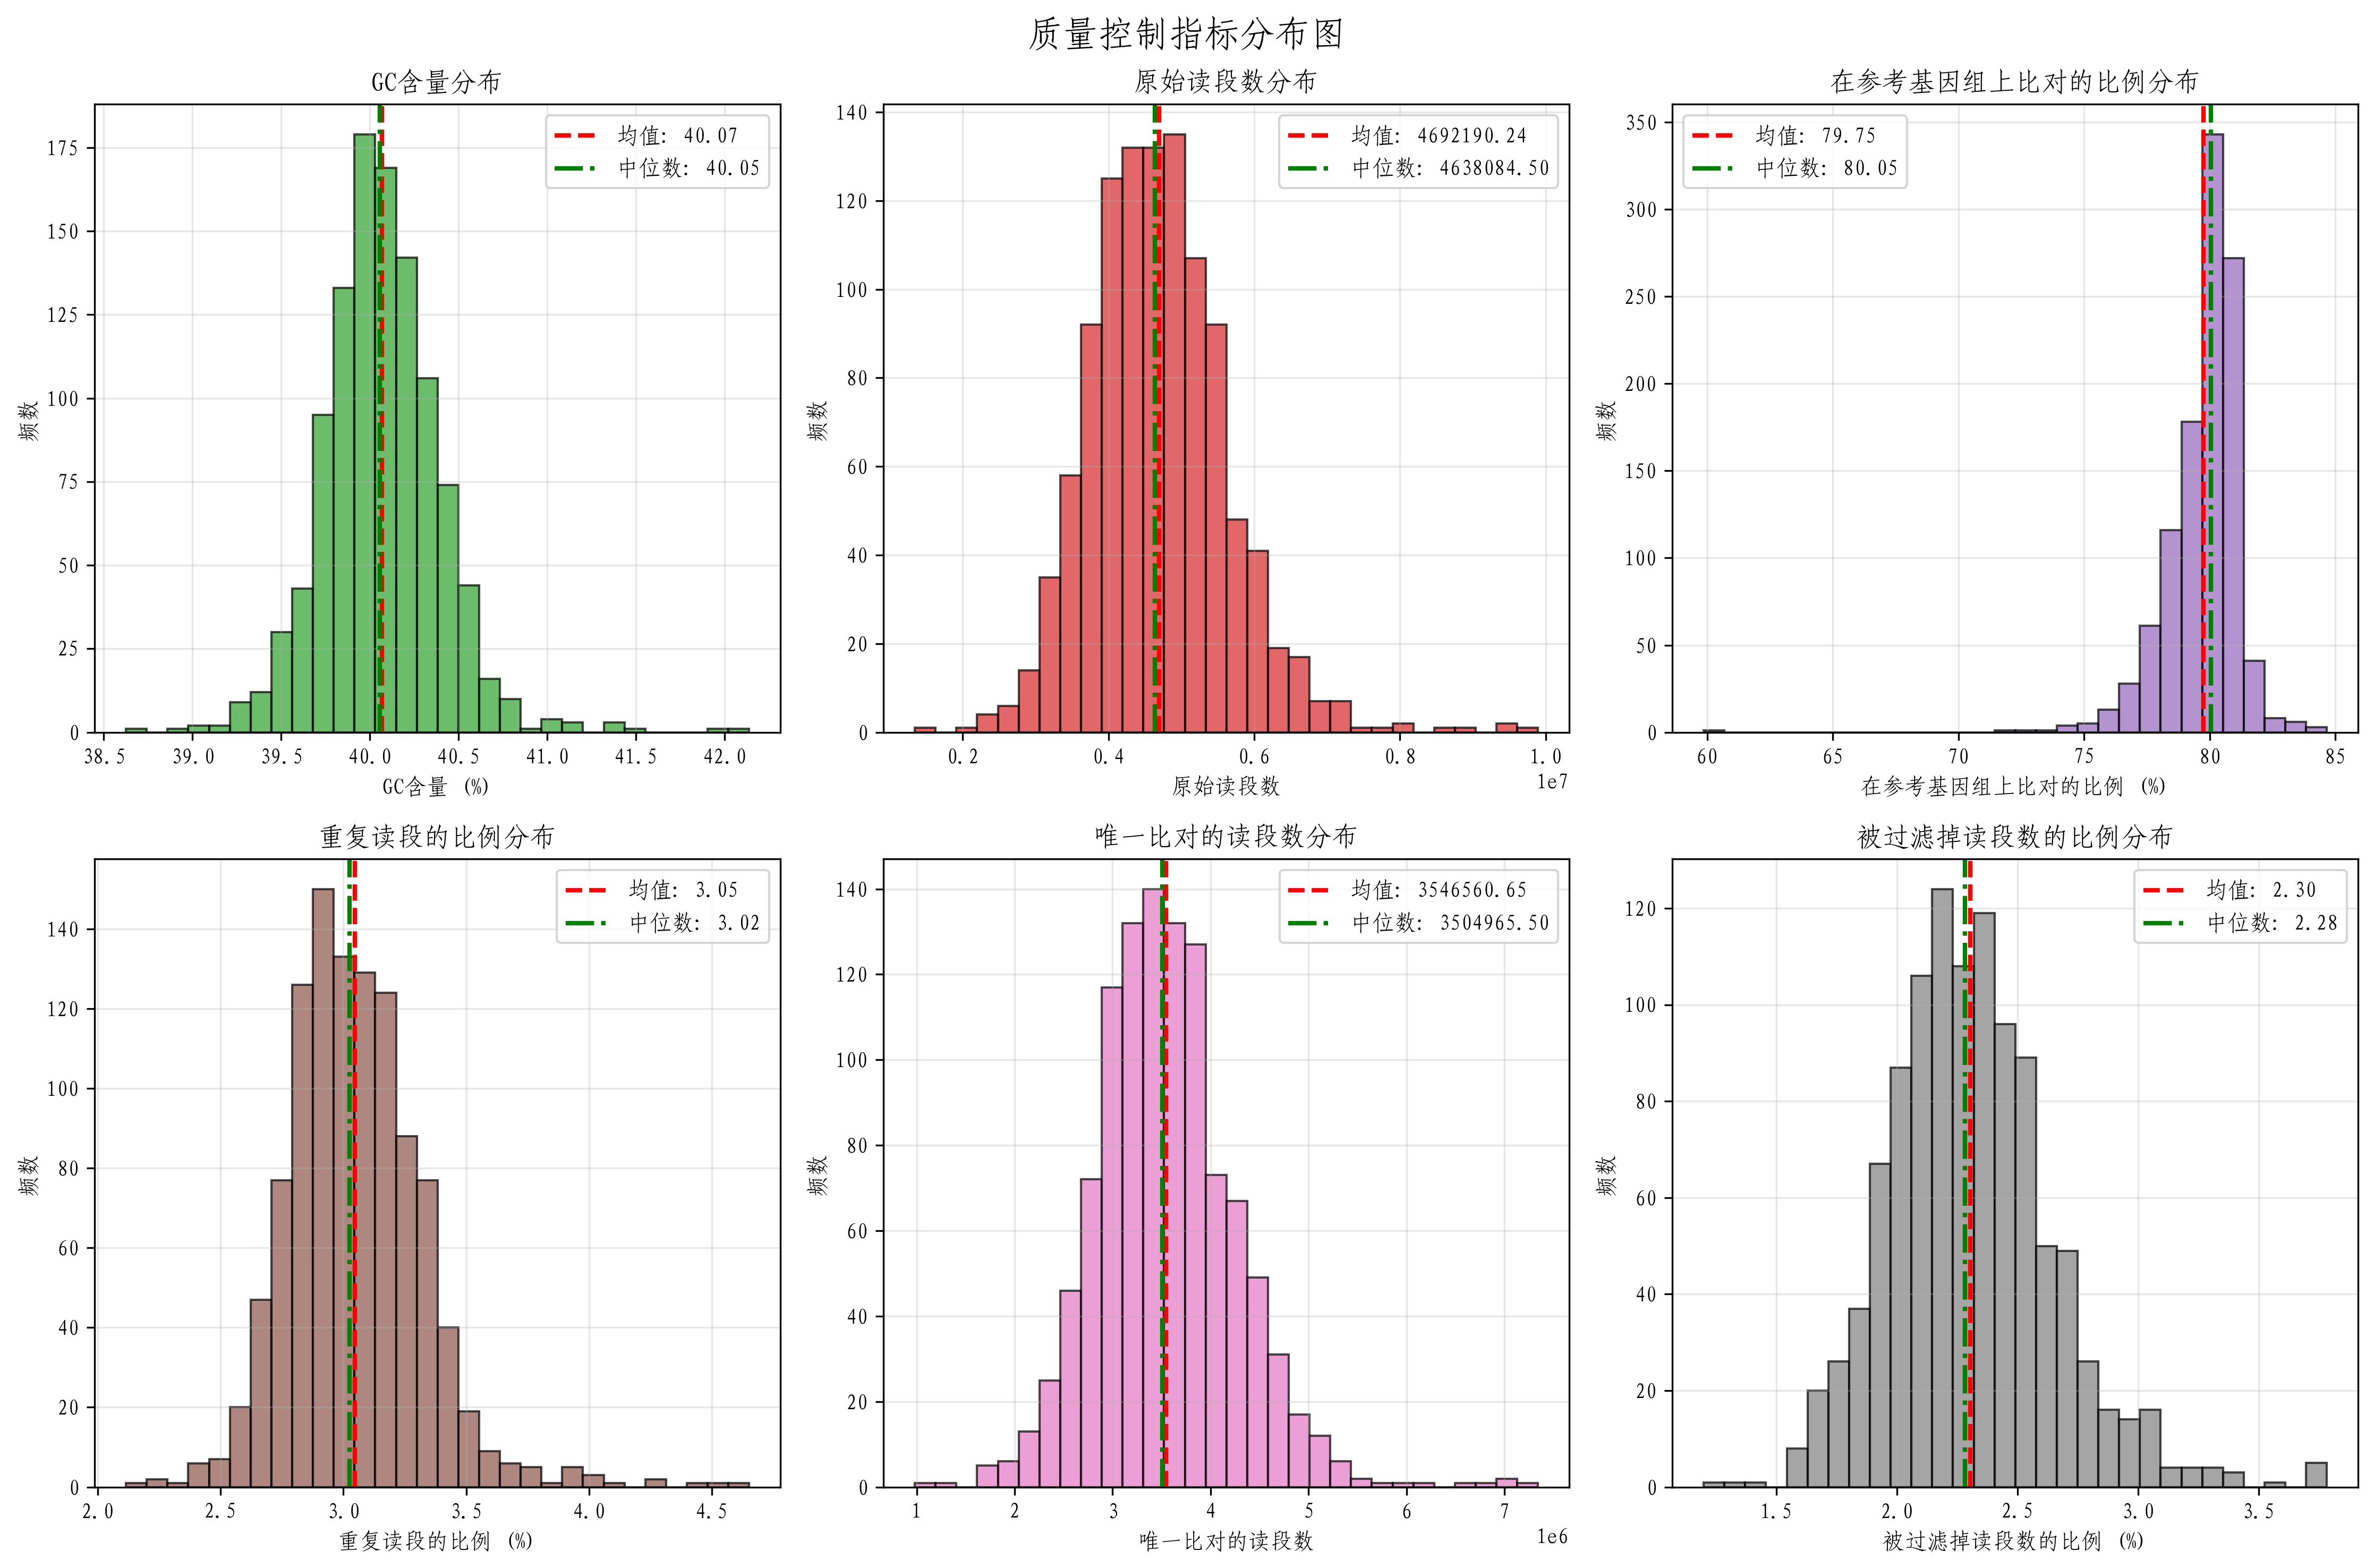
\includegraphics[width=0.8\textwidth]{../figure/q1_质量控制指标分布图.png.png}
    \caption{}
    \label{fig:heatmap}
\end{figure}

\subsection{问题二模型的建立与求解}

\subsection{问题三模型的建立与求解}

\subsection{问题四模型的建立与求解}

% 模型评价
\section{模型评价}
\subsection{模型优点}

\subsection{模型缺点}

% 摘要
\bibliography{ref}

% 附录

\begin{appendices}
    % \section{附录名}
\end{appendices}

\end{document}